\chapter{Analiza danych Big Data}

Termin \textit{Big Data} odnosi się do dużych, zmiennych i różnorodnych zbiorów danych, których przetwarzanie i analiza jest pracochłonne, ale może prowadzić do ciekawych wniosków oraz pozyskania nowej wiedzy. Zbieranie oraz przechowywanie dużej ilości danych do analizy było praktykowane od bardzo dawna, jednak dokładniejsza koncepcja Big Data została poznana w 2001 roku kiedy to analityk Doug Laney zaprezezentował znaną dzisiaj definicję \textit{3V}: \textit{volume}, \textit{velocity}, \textit{variety} czyli: ilość, szybkość, złożoność, a później dodano jeszcze czwarty atrybut \textit{veracity} czyli: wiarygodność.

\section{Pojęcie Big Data}
Wraz ze wzrostem zainteresowania Big Data podjęto próby dokładniejszego opisania tego terminu. Obecnie definiując to pojęcie trzeba odnieść się do nowych rozwiązań technologicznych dotyczących wielkich wolumenów danych o innym charakterze ilościowym oraz jakościowym niż dotychczas. \\
Jedna z pierwszych definicji Big Data została zaprezentowana przez M. Cox i D. Ellsworth w 1997 r. jako duża ilość danych, którą należy zwiększać, aby wydobyć wartości informacyjne. Inna i najbardziej popularna, została przestawiona w 2001 r. przez pracującego dla firmy analityczno-doradczej wspomnianego analityka D. Laney, opiera się o trzy atrybuty: ilość, szybkość i złożoność. W 2012 r. ta sama firma dodała do swojej definicji kolejne dwa atrybuty: zmienność i złożoność. Autorzy innej publikacji \textit{Big Data: Issues, Challenges, Tools and Good Practices} z 2013 r. definiują pojęcie Big Data jako wymagające stosowania nowych technologii i architektur z powodu potrzeby ekstrakcji wartości płynącej z tych danych. \\
Podsumowując, określenie Big Data to pojęcie odnoszące się do zbiorów danych, które jednocześnie charakteryzują się dużą objętością, różnorodnością, strumieniowym napływem w czasie rzeczywistym, zmiennością, złożonością oraz wymagają stosowania innowacyjnych technologii i narzędzi, aby możliwe było wydobycie z nich wartościowych informacji.

\begin{figure}[h] % h means here
	\centering
	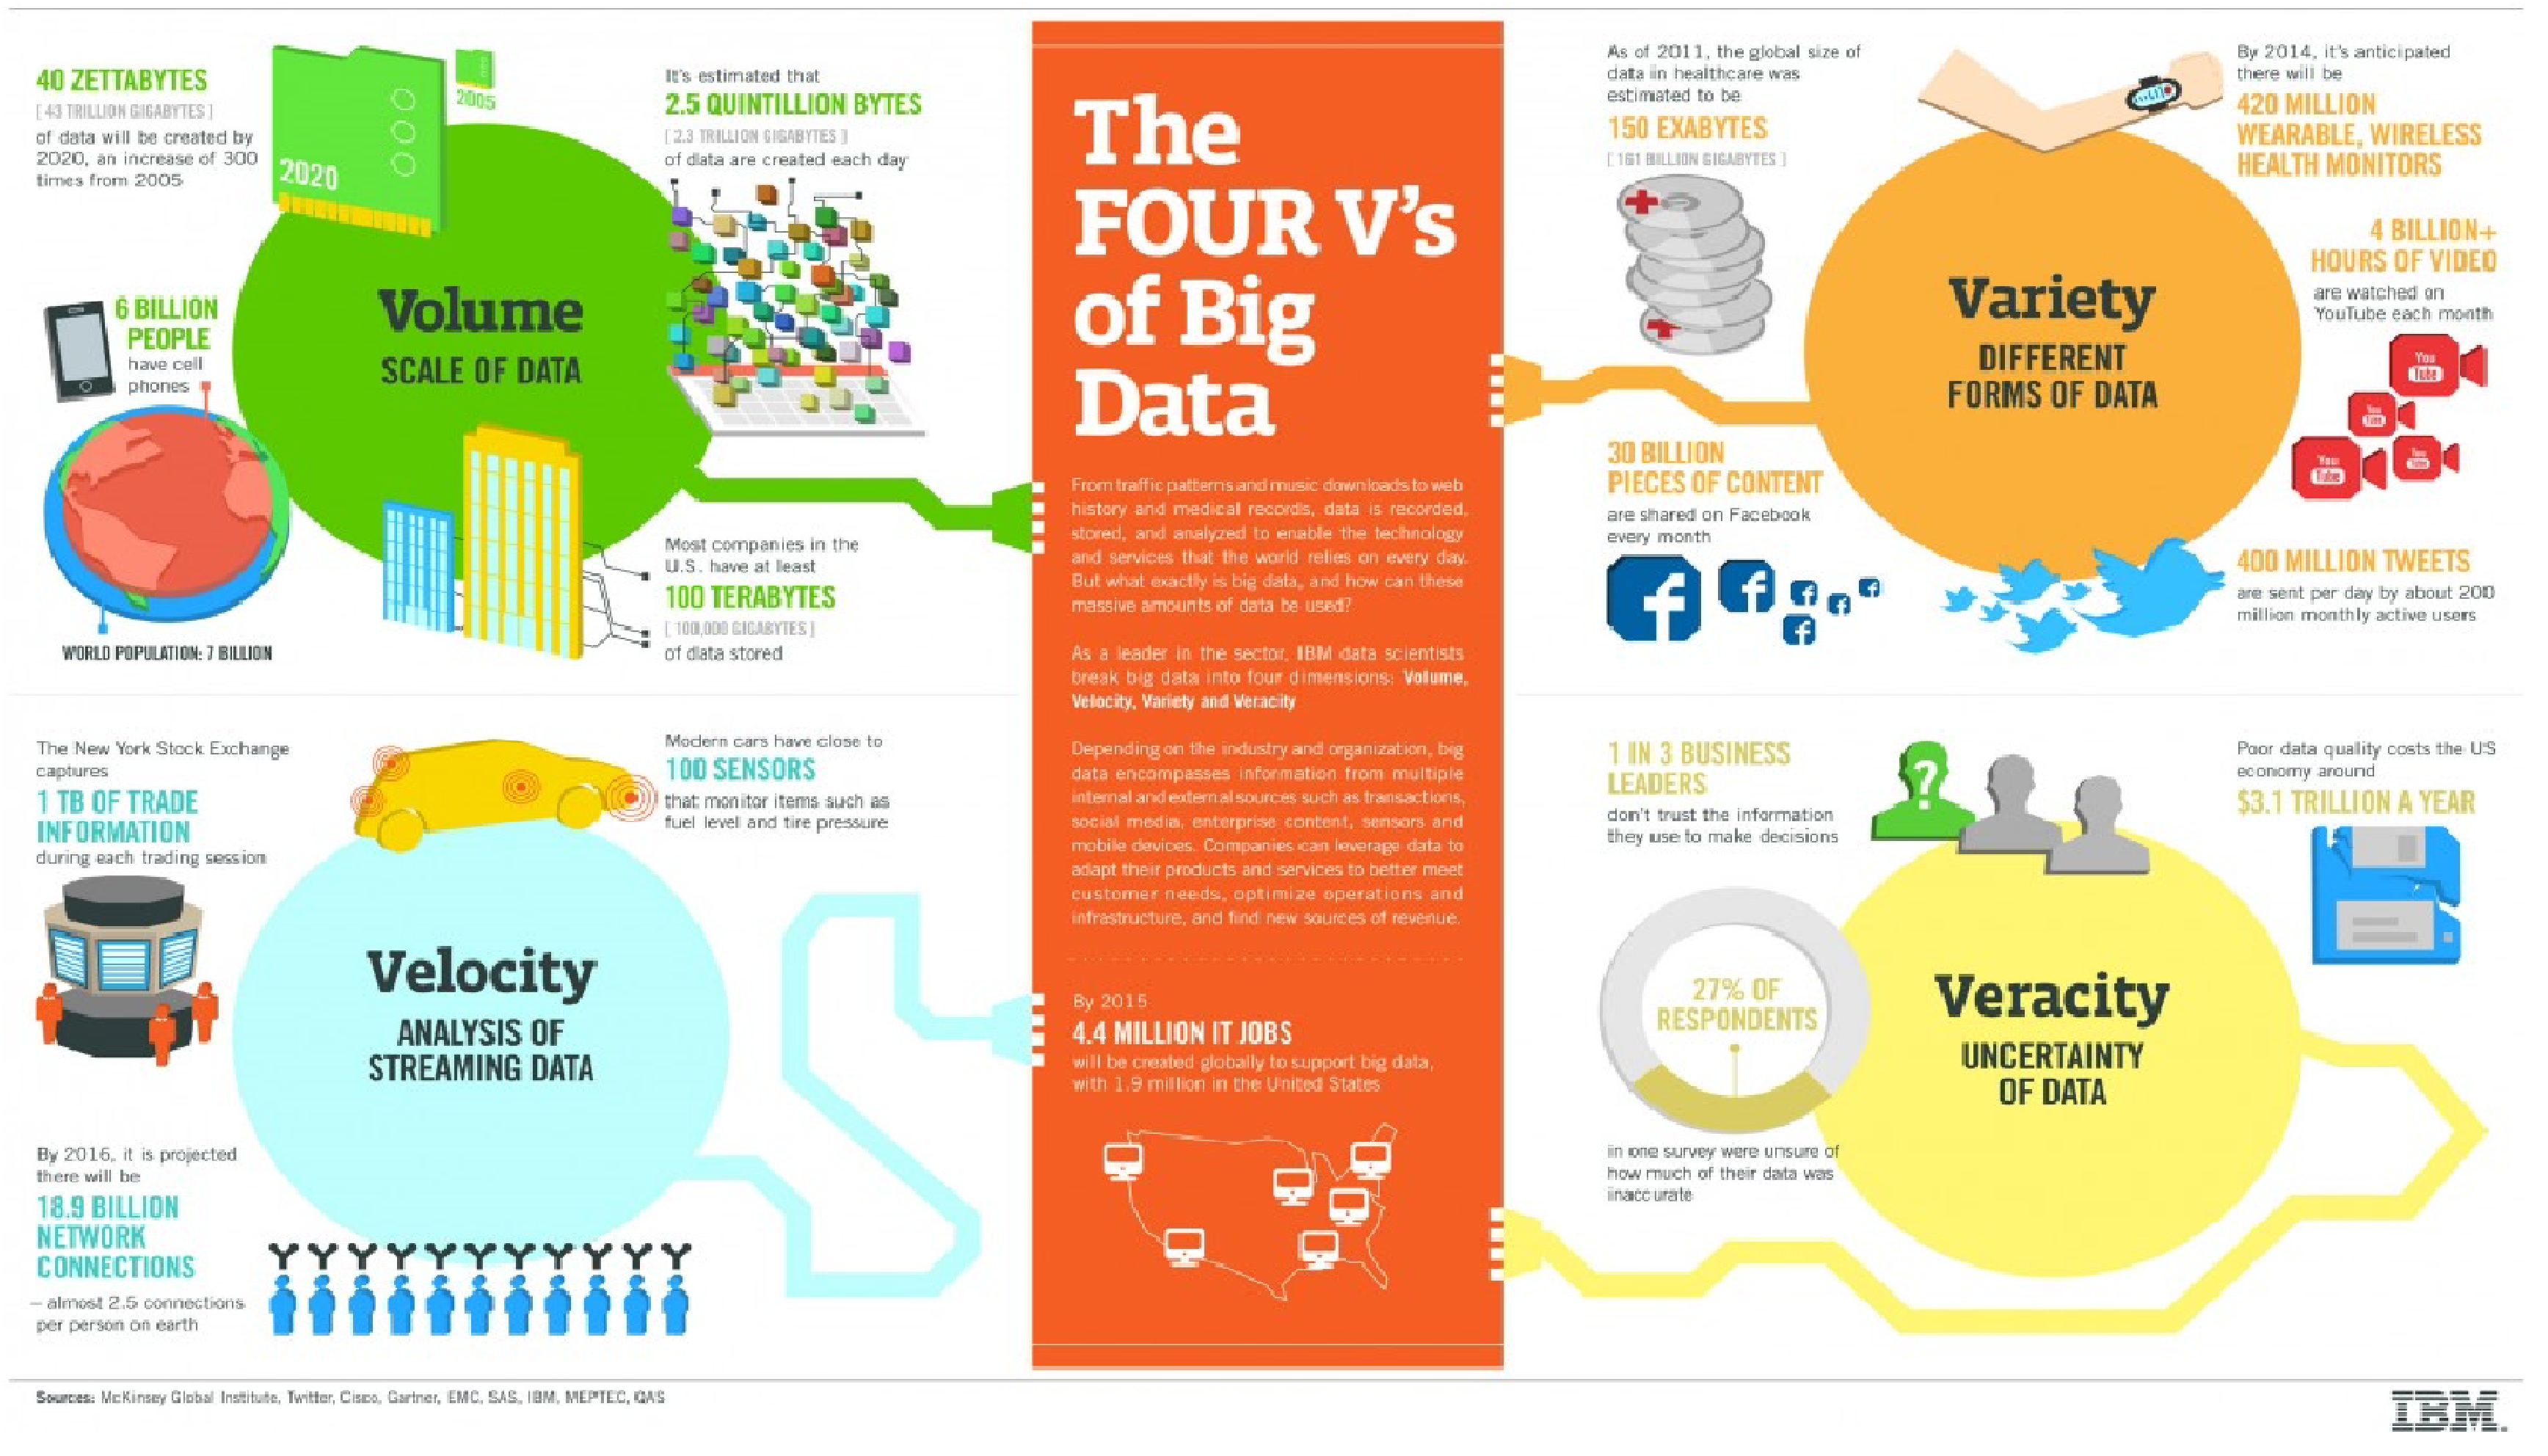
\includegraphics[width=1.0\linewidth]{img/big_data_4_v}
	\caption{Definicja \textit{Big Data} w ujęciu 4V.}
\end{figure}

\section{Charakterystyka}
Termin Big Data charakteryzują atrybuty: objętość, szybkość, różnorodność, zmienność, złożoność i wartość. W dalszej cześci tej pracy dyplomowej przedstawiono omówienie każdego z tych atrybutów.

\subsection{Objętość}
Atrybut ten odnosi się do dużej ilości danych, które wymagają nowych technologii. Rozmiar danych zależy od dziedziny i może wynosić od terabajtów lub petabajtów w zagadnieniach takich jak np. analiza zderzeń cząstek elementarnych w fizyce do megabajtów lub gigabajtów np. w telekomunikacji przy analizie połączeń wykonywanych przez abonentów. Najnowsze badania prognozują, że ilość danych wzrośnie do 2020 r. o 40\% zeta bajtów, co będzie skutkować 50-krotnym wzrostem od początku 2010 r..

\subsection{Szybkość}
Duża szybkość napływających danych charakteryzuje się strumieniowym napływem wymagającym analizy w czasie rzeczywistym. Z powodu ograniczeń przepustowości sieci dane takie należy pobierać porcjami i filtrować pod kątem przydatności oraz wartości informacji jaką ze sobą niosą.

\subsection{Różnorodność i złożoność}
Kolejne atrybuty czyli różnorodność i złożoność są ze sobą powiązane i odnoszą się do dużego zróżnicowania źródeł pochodzenia danych i ich formatu. Informacje mogą przychodzić w postaci ustrukturyzowanej jak i m.in. niestrukturalnych dokumentów tekstowych, wiadomości e-mail, materiałów audio i video, transakcji finansowych. Natomiast źródłami ich pochodzenia mogą być wszystkie systemy, które generują i gromadzą dane czyli np.: 

\begin{itemize}
	\item[--] wewnętrzne systemy organizacji takie jak systemy księgowe, kadrowe i transakcyjne,
	\item[--] źródła zewnętrzne - dane ze stron internetowych (także te nieindeksowane przez wyszukiwarki - pochodzące z głębokiego internetu), blogów, wiadomości tweet i forów internetowych,
	\item [--] sklepy, usługodawcy i instytucje finansowe,
	\item[--] instytucje zdrowia.
\end{itemize}

\subsection{Zmienność}
Dane typu Big Data podlegają okresowym trendom i wahaniom. Napływają ze zmiennym w czasie natężeniem. Mają na to wpływ wydarzenia z wielu dziedzin naszego życia - od pór roku do wydarzeń z dziedziny polityki czy sportu. Przykładem jest np. zainteresowanie inną tematyką w czasie Bożego Narodzenia niż w czasie lata lub bardziej dynamiczne zmiany na rynkach finansowych.

\subsection{Wartość}
Wartość danych napływających z systemów jest trudna do analizy, ponieważ struktura tych danych charakteryzuje się dużą złożonością, a korzyść płynąca z analizy jest ukryta. Obecnie istnieją już systemy, które potrafią radzić sobie z dużym wolumenem informacji, ale to jak te informacje zostaną wykorzystane zależy już od człowieka.

\section{Paradygmat MapReduce}
Większość systemów przetwarzających duże ilości danych opiera swoje działanie o paradygmat \textit{MapReduce}. MapReduce polega na dzieleniu zbioru danych wejściowych na mniejsze niezależne od siebie podzbiory, które są następnie przetwarzane przez równoległe zadania typu \textit{map}. Wynik wyjścia z zadań typu map jest sortowany, a następnie podawany na wejście zadań typu \textit{reduce}. Zastosowanie tego paradygmatu skutkuje zwiększeniem wydajności dzięki przetwarzaniu równoległemu niezależnych bloków danych co może zostać wykorzystane przez zastosowanie wielu procesorów.\\
MapReduce przetwarza wyłącznie pary \textit{<klucz, wartość>}. Dlatego większość operacji polega na znalezieniu elementów spełniających pewne kryteria, umieszczenie ich w zbiorze oraz zwiększenie licznika sygnalizującego częstotliwość występowania elementu tak jak pokazano na ilustracji 4.2..

\begin{figure}[h] % h means here
	\centering
	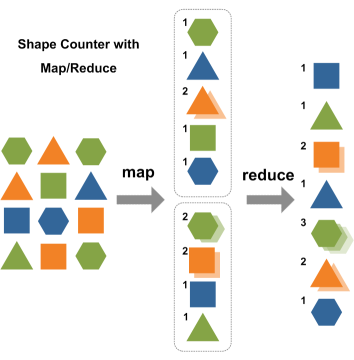
\includegraphics[width=0.6\linewidth]{img/big_data_mapreduce}
	\caption{Przykład zastosowania paradygmatu \textit{MapReduce}.}
\end{figure}

\section{Wymagania stawiane przed systemami Big Data}
Przetwarzanie danych napływających w sposób strumieniowy wiąże się z dużym wyzwaniem związanym z koniecznością niezwłocznej obsługi danych pojawiających się w dużej ilości i z dużą prędkością. Są to wymagania stawiane przede wszystkim przed platformami zarządzania danymi - ich przetwarzaniem oraz przechowywaniem. Jednymi z najbardziej znanych obecnie rozwiązań tego typu są \textit{Apache Hadoop} oraz \textit{Apache Spark}, które zostaną omówione w dalszej części pracy przy okazji sformułowania wymagań stawianych przed aplikacją zbudowaną na potrzeby tej pracy dyplomowej i dostępnych rozwiązań. \\
Innym napotkanym problemem jest duża złożoność danych, szczególnie danych niestrukturalnych, która stawia wyzwania związane z efektywnym przechowywaniem informacji oraz przeszukiwaniem bazy danych. Sztywno zdefiniowane relacyne bazy danych nie odpowiadają wymaganiom stawianym przed systemami Big Data. Bazami, które znalazły swoje zastosowanie w takich systemach są bazy \textit{NoSQL}. Dzięki ich zastosowaniu można uzyskać korzyści związane z poprawą zrozumienia danych, możliwość gromadzenia danych niestrukturalnych, skalowalność oraz elastyczność bazy danych. Przykładem baz danych typu NoSQL są \textit{Cassandra} oraz \textit{Neo4j}, które tak jak i Apache Hadoop oraz Apache Spark zostaną omówione w dalszej części pracy.

\begin{figure}[h] % h means here
	\centering
	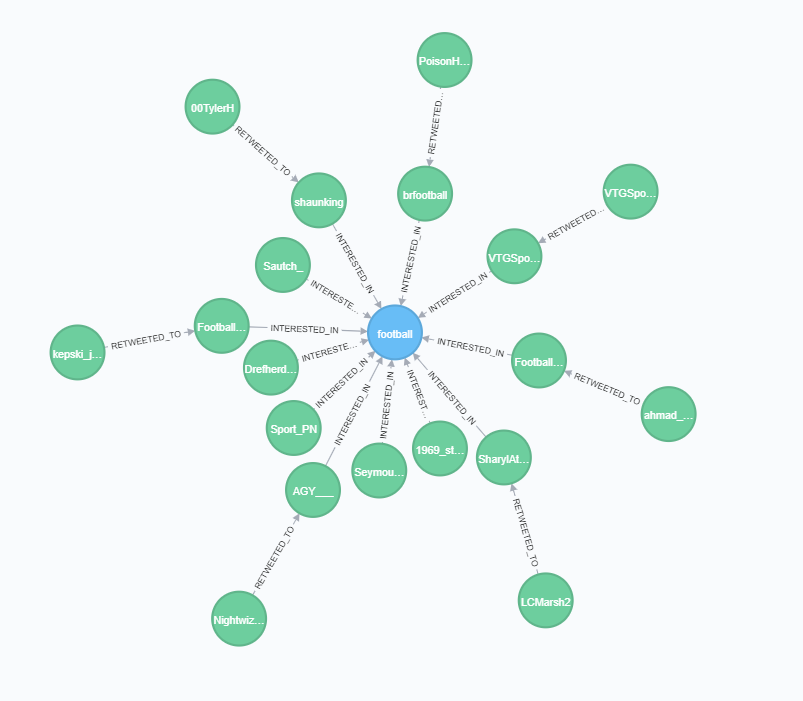
\includegraphics[width=0.8\linewidth]{img/big_data_neo4j}
	\caption{Przykład zastosowania grafowej bazy danych Neo4j.}
\end{figure}

\section{Przykłady zastosowania systemów Big Data}
Systemy Big Data mogą mieć bardzo szerokie zastosowanie. Poniżej podano listę istniejących już zastosowań, są to np.:

\begin{itemize}
	\item[--] wykorzystanie danych pogodowych generowanych przez Interdyscyplinarne Centrum Modelowania Matematycznego i Komputerowego ICM Uniwersytetu Warszawskiego do m.in. prognozowania ilości energii produkowanej przez elektrownie wiatrowe i słoneczne, prognozowania zagęszczenia ruchu, pomoc sieciom handlowym w prognozowaniu jakie produkty będą się lepiej sprzedawały i powinny być w promocyjnej cenie, 
	\item[--] wykorzystanie zegarków, należących do układów typu wearables, wraz z smartfonami oraz systemów Big Data do analizy zdrowia pacjenta np. przy leczeniu choroby Parkinsona, ale też w innych chorobach gdzie ważne jest codzienne monitorowanie,

\begin{figure}[h] % h means here
	\centering
	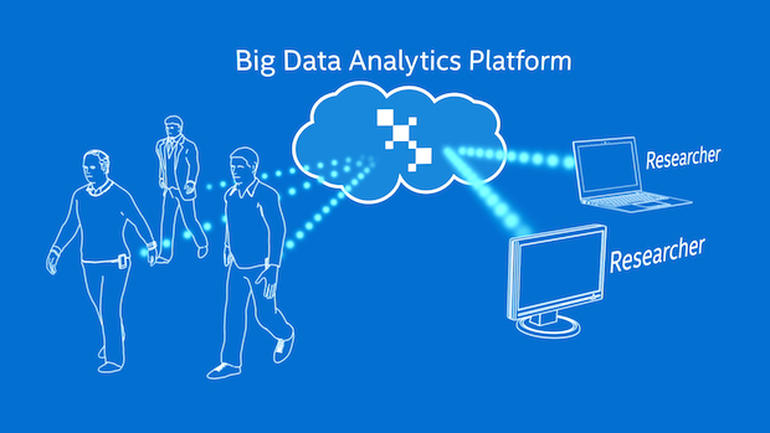
\includegraphics[width=0.6\linewidth]{img/big_data_intel_parkinson}
	\caption{Przykład zastosowania układów wearables, telefonów komórkowych i systemu Big Data do analizy stanu zdrowia pacjentów.}
\end{figure}

	\item[--] dzięki zbieraniu i analizie danych takich jak np. temperatura, czas otwarcia drzwi, ilość kursów z wind oraz specyfikacji sprzętu przewidywany jest czas kiedy należy wykonać naprawę, a służby serwisowe wysyłane są tylko wtedy i tylko tam gdzie są rzeczywiście potrzebne,
	\item[--] gromadzenie danych ze stron internetowych wraz z wyrażanymi przez internautów opiniami i analiza ich za pomocą systemów wykorzystujących sztuczną inteligencję służy firmom, ale także partiom politycznym, do monitorowania opinii na temat produktów oraz nastrojów społecznych.
	
\end{itemize}

